% Un tutorial
% https://www.overleaf.com/learn/latex/How_to_Write_a_Thesis_in_LaTeX_(Part_1):_Basic_Structure
% -----------------------------------------------------------------------------
% Paquetes y configuracion
% -----------------------------------------------------------------------------
\documentclass[11pt,twoside]{report}
\usepackage[utf8]{inputenc}
\usepackage[spanish]{babel}
\usepackage[a4paper,width=170mm,top=25mm,bottom=25mm,bindingoffset=6mm]{geometry}
\usepackage{fancyhdr}
\usepackage[backend=biber]{biblatex}  % bibliografia
\usepackage{csquotes}
\usepackage{graphicx}

\usepackage{longtable}
\usepackage[acronym]{glossaries} % nomenclatura y abreviaciones
% Abreviaciones
\newacronym{ag}{AG}{Algoritmo genético}
\newacronym{mrcvc}{MRCVC}{Motor rotativo de combustión a volumen constante}
\newacronym{rans}{RANS}{\emph{Reynolds-average Navier-Stokes}}
\newacronym{dta}{DTA}{Diámetro del tubo de admisión}
\newacronym{dte}{DTE}{Diámetro del tubo de escape}
\newacronym{lta}{LTA}{Longitud del tubo de admisión}
\newacronym{lte}{LTE}{Longitud del tubo de escape}
\newacronym{iia}{IIA}{Ángulo de apertura del puerto de admisión}
\newacronym{ifa}{IFA}{Ángulo de cierre del puerto de admisión}
\newacronym{eia}{EIA}{Ángulo de apertura del puerto de escape}
\newacronym{efa}{EFA}{Ángulo de cierre del puerto de escape}
\newacronym{unl}{UNL}{Universidad Nacional del Litoral}
\newacronym{unco}{UNCo}{Universidad Nacional del Comahue}

% Nomenclatura
\newglossaryentry{reynolds}{
    name = $R_e$ ,
    description = Número de Reynolds
}
\newglossaryentry{rend_vol}{
    name = $\eta_v$ ,
    description = Rendimiento volumétrico
}
\newglossaryentry{dens_atmo}{
    name = $\rho_{a,i$ },
    description = Densidad del aire atmosférico
    }
\newglossaryentry{vel}{
    name = $V$ ,
    description = Velocidad
}
\newglossaryentry{ang_ciclo}{
    name = $\theta_c$ ,
    description = Ángulo de ciclo
}
\newglossaryentry{ang_cig}{
    name = $\theta_g$ ,
    description = Ángulo del cigüeñal
}

  % esto esta mejor si lo pongo en cada entrada de texto
\makeglossaries

\graphicspath{ {figuras/} }
\addbibresource{bib.bib}

\pagenumbering{roman}

\fancyhead{}
\fancyhead[RO,LE]{Proyecto Integrador Profesional}
\fancyfoot{}
\fancyfoot[LE,RO]{\thepage}
\fancyfoot[LO,CE]{Capítulo \thechapter}
\fancyfoot[CO,RE]{Nicolás Daniel Barrios}

% -----------------------------------------------------------------------------
% Documento
% -----------------------------------------------------------------------------
\begin{document}

% -- Iniciales
\begin{titlepage}
    \begin{center}

        \vspace*{2cm}
        \huge
        \MakeUppercase{\textbf{Diseño de los sistemas de admisión y escape del
        Motor Rotativo de Combustión a Volumen Constante }}

        \vspace{0.8cm}
        Nicolás Daniel Barrios
        \vfill

        \vspace{0.8cm}
        
\includegraphics[width=0.5\textwidth]{logo_unco.jpg}
        \vspace{0.8cm}


        \large
        Facultad de Ingeniería \\
        Universidad Nacional del Comahue \\
        Argentina \\
        2021
    \end{center}
\end{titlepage}

\setcounter{page}{1}
\section*{Agradecimientos}
A mi familia y amigos.

\section*{Resumen}
Aca un pequeño resumen.

\tableofcontents
\listoffigures
\listoftables
\printglossary[type=\acronymtype,title=Abreviaciones]
\printglossary[title=Nomenclatura]

% -- Cuerpo del texto
\pagenumbering{arabic}
\chapter{Introducción}

Este trabajo presenta un procedimiento para optimizar la geometría del sistema
de intercambio de gases del \gls{mrcvc}
\cite{toth}, en particular de la geometría y posición en el cuerpo estatórico
de los puertos de admisón y escape, diámetro y longitud de los conductos
corresponidentes.

El MRCVC es un proyecto nacido en la Universidad Nacional del Comahue en el
marco del \emph{Proyecto de Investigación Desarrollo de modelos y herramientas
para la simulación de problemas complejos en ingeniería mediante
fluidodinámica computacional (04/I-251)}. Actualmente se encuentra en etapa
de desarrollo.

La optimización de la geometría se realizó con un conjunto de herramientas, en
primer lugar para obtener las curvas de redimiento volumétrico se utilizó un
simulador de motores de combustión interna, 

Se utilizó un simulador de motores de combustión interna para simular obtener
las curvas características del motor, curvas que se utilizan para dar un
puntaje a una algoritmo genético para optimizar el conjunto de parámetros que
definen la geometría de los sistemas de intercambio de gases y 

La motivación de este trabajo surge de continuar con el desarrollo del Motor
Rotativo de Combustión a Volumen Constante (MRCVC), en particular
mejorar el prediseño de los sistemas de intercambio de gases sentando las bases
para una futura optimización de los mismos en un motor con requisitos de diseño
establecidos.

\chapter{Antecedentes} \label{cap:antecedentes}

\section{Motor Rotativo de Combustión a Volumen Constante}
%
El MRCVC es un proyecto que surgió en la Universidad Nacional del
Comahue, inventado y patentado en el año 2004 por Jorge Toth\cite{toth}.
%
Actualmente se encuetra en desarrollo en el Departamento de Mecánica Aplicada
de la UNCo, en el marco del Proyecto de Investigación Desarrollo de modelos y
herramientas para la simulación de problemas complejos en ingeniería mediante
fluidodinámica computacional (04/I-251).

En trabajos anteriores\cite{lopez16, lopez13, roldan} se han mencionado las
características que hacen al MRCVC un motor atractivo. La geometría de la cámara
de combustión y del conjunto rotante permiten  combustión a volumen constante y
un balanceo mecánico de fuerzas.
%
Esto permite un funcionamiento más suave del motor, además de una reducción del
ruido y desgaste en comparación a motores rotativos tradicionales (Wankel) y
alternativos.


No obstante a esto hay que mencionar que los motores rotativos traen consigo una
serie de problemas como la necesidad de introducir aceite a la cámara de
combustión para lubricar elementos móviles, el solape de cámaras durante la
apertura de los puertos y en particular al MRCVC un complejo sistema de
sellos\cite{roldan}.



\section{Sistema de Intercambio de Gases}
%
Este sistema cumple la función de extraer los gases quemados de la cámara de
combustión de manera eficiente al final de cada carrera de expansión y de
admitir una carga de mezcla fresca para el próximo ciclo.
%
% En un motor de cuatro tiempos, el sistema suele estar compuesto por un filtro
% de aire,  tubo que conecta el filtro con el cuerpo de mariposa, cuerpo de
% mariposa, plenum de admisión y un puerto de admisión, como se ve en la
% figura \ref{fig:sist_intercambio}.
%
La masa de aire inductada imita la cantidad de combustible que se puede quemar,
por este motivo es importante tener un sistema de admisión eficiente.
%
De la misma manera, la cantidad de gases quemados que se pueden extraer luego de
cada ciclo limita la cantidad de masa fresca que puede ingresar a la cámara de
combustión.
%
Otros objetivos del sistema de intercambio de gases son el de preparar la
mezcla\footnote{En el caso de motores SI que admiten mezclas de aire y
combustible} y brindar un flujo que favorezca el proceso de combustión.

% \begin{figure}[h!] \centering
% 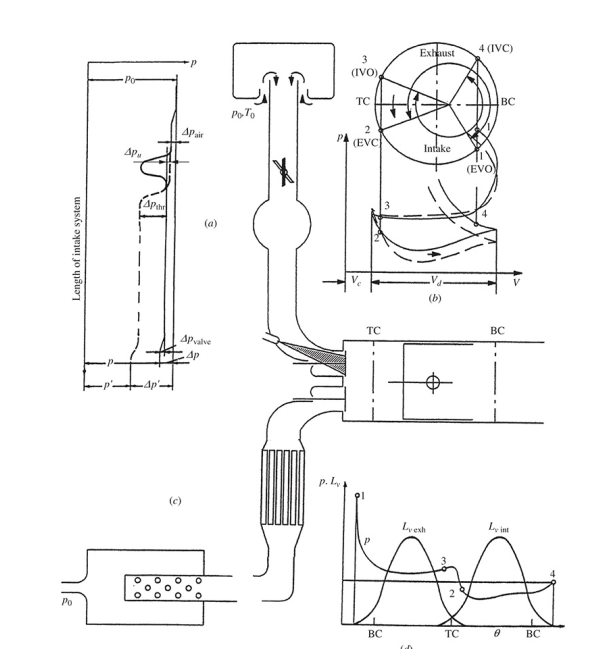
\includegraphics[width=0.5\textwidth]{sistema_intercambio_gases.png}
% \caption{Sistema de intercambio de gases esquematizado(buscar una libre o hacer
% un esquema propio)} \label{fig:sist_intercambio} \end{figure}

Para la simulación del MRCVC se usa una sistema simplificado, que consta de un
tubo de diámetro $D$ y longitud $L$ tanto para la admisión como para el escape,
como se ilustra en la figura \ref{fig:sist_int_mrcvc}.
%
La apertura y cierre de los puertos es controlada por la posición angular de los
puertos en el estator.

% \subsection{Solape de cámaras}
% %
% Es un proceso que ocurre en ambos puertos y que debe ser tenido en cuenta a la
% hora de evaluar el comportamiento del sistema de admisión y escape.
% %

\subsection{Indicadores de rendimiento}

Se medirá la eficiencia del sistema de intercambio de gases utilizando
exclusivamente el rendimiento volumétrico, $\eta_v$.
% Los conductos de admisión restringen el flujo de aire hacia el motor, para
% medir la eficiencia con la que se está admitiendo aire al motor se define el
% rendimiento volumétrico $\eta_v$.
%
Este se define como la relación entre el caudal volumétrico de aire que ingresa
al sistema de admisión y la velocidad a la que cambia el volumen dentro de un
cilindro.


\begin{equation}
  \label{eq:rendVol}
  \eta_v = \frac{2 \dot{m}_a}{\rho_{a,i} V_d N}
\end{equation}

Donde: $\rho_{a,i}$ es la densidad del aire a la entrada del sistema de
admisión (para motores naturalmente aspirados). También se puede definir
$\eta_v$ como:

\begin{equation}
    \label{eq:rendVol2}
    \eta_v = \frac{m_a}{\rho_{a,i} V_d}
\end{equation}

Dónde $m_a$ es la masa inductada al cilindro en cada ciclo.

Hay varios factores que afectan al rendimiento volumétrico, entre los más
importantes están:
%
\begin{enumerate}
    %
    \item Efectos cuasiestáticos
    %
    \item Pérdidas de carga por fricción viscosa
    %
    \item Pérdidas de carga en los puertos de admisión y escape
    %
    \item Transferencia de calor en sistema de admisión
    %
    \item Reglaje de los válvulas/puertos
    %
    \item Bloqueos de flujo en puertos de admisión y escape
    %
    \item Transferencia de calor en el cilindro
    %
    \item Sintonía del puerto de admisión y escape
    %
    \item Métodos de sobrecarga 
\end{enumerate}

Para este trabajo es de interés particular la pérdida de carga en los puertos,
el reglaje y la sintonía de admisión y escape.
%
En \cite{lopez13} se demostró que se tiene una mejor \emph{performance} del
motor si se ubican los puertos en el cuerpo central del estator, realizando un
optimización de la geometría mediante un barrido paramétrico de las variables
geométricas que determinan la forma, posición y reglaje de los puertos.
%
% La ubicación angular de los puertos determina la duración de los procesos de
% admisión y escape, además de modificar la forma y el coeficiente de descarga.

Estos parámetros se ajustan o seleccionan teniendo en cuenta requisitos de
funcionamiento del motor, por lo que fue necesario establecer una curva de
rendimiento volumétrico para que la simulación numérica del
ciclo termodinámico se pueda acoplar al algoritmo de optimización y de este
modo evaluar los motores contra la curva de rendimiento requerida.
%
El criterio de diseño/selección de la curva de $\eta_v$ fué el siguiente:

\begin{itemize}
  \item que tenga un pico de rendimiento entre 4000 y 6000 rpm.
  \item que la curva sea suave
\end{itemize}

% \subsubsection{Fracción de gases residuales}
% %
% A diferencia de un motor alternativo convencional en el que, por medio de
% métodos de sobrecarga se podría reducir la cantidad de gases residuales a una
% fracción despreciable, en el MRCVC, dada la disposición de la geometría siempre
% se transfiere gas residual desde una cámara que está transcurriendo por el
% barrido a la cámara contigua que está iniciando el proceso de admisión.

% Esta masa residual se puede calcular y depende del volumen atrapado y la preisón
% cuando cierra el puerto de escape.
% %
% Esta masa residual marca una cota inferior a la fracción de gases residuales
% que se pueden obtener, se menciona esto porque es un indicador del rendimiento
% de los sistemas de intercabmio de gases.
% %
% Considerando un motor con geometría perfecta y sin pérdida de masa entre los
% sellos, $x_{r\ min}$ se puede calcular como:

% $$
% x_{r\ min} = 0
% $$

% Considerando los valores gemoétricos utilizados para realizar esta optimización,
% este valor de $x_{r\ min}=0.1$ representa un objetivo para este trabajo.

% \subsection{Flujo a través de las válvulas}
% %
% Durante el escape, el soplido es un proceso que puede favorecer a la descarga
% de una cámara.

\subsection{Estrategias de simulación de motores}
%
Se simulará el motor con el simulador de motores de combustión interna ICEsym,
este simulador utiliza modelos 0D para la combustión y 1D para el flujo de
gases a través de los conductos (fuera de la cámara de combustión).

Esta es una herramienta muy útil ya que permite evaluar la \emph{performance} de
un motor a un costo computacional bajo además, la manera en que se implementó la
entrada y salida de datos permite utilizar este simulador como una ``caja
negra'' de modo que se pudo implementar en un \emph{script} como una función a
la que se le otorga como entrada un conjunto de parámetros y devuelve los
resultados de la simulación en un formato que permite la lectura y evaluación de
los mismos.
%
Esta característica del programa la que permitió acoplarlo con un algoritmo
genético para realizar la optimización de la geometría.


Como se mencionó en el apartado \ref{sec:rend_vol}, en trabajos previos se
realizó un pre diseño de los puertos de admisión y escape.
%
En dicho trabajo se determinó coeficientes de descarga constantes
% En dicho trabajo se utilizaron coeficientes de descarga estimados y constantes
para simular el flujo en los puertos de admisión y escape.
%
Con el objetivo de modelar con mayor precisión el flujo a través de los puertos
se realizó una modificación al código de ICESym que permite utilizar una
variable adicional para modelar al $C_d$, con lo que se puede representar la
dependencia con la apertura del puerto como con la diferencia de presión
instantánea como $C_d = f(lv, \delta P)$.

% Heywood 2Ed, pag 376
\chapter{Análisis del problema}

\section{Optimización de la geometría}

\subsection{Simulación computacional del ciclo termodinámico MRCVC}

\subsubsection{ICESym}

ICESym \cite{icesym} es un simulador de motores de combustión interna
desarrollado en conjunto por la UNCo y UNL, utiliza modelos unidimensionales
para simular el flujo en los conductos de admisión y escape y modelos cero
dimensionales para el resto de los componentes.

El simulador incluye un modelo para el solape entre cámaras \cite{lopez16} y
modificaciones particulares al MRCVC, para este trabajo en particular  y con el
fin de obtener una mapa del coeficiente de descarga, se ha agregando la
diferencia de presión entre cámara y puerto como variable de modo que $Cd =
f(L_v, \delta P)$.

La combustión se realiza a volumen constante, por lo que es de esperarse
mayores rendimientos de conversión de combustible en relación a motores en los
que la combustión no se realiza a volumen constante.
% hace falta mostrar que esto es así? poner algún gráfico del heywood o cosas
% por el estilo. puedo citar el heywood?

El indicador que se tomará como referencia para evaluar y comparar diferentes
geometrías es el rendimiento volumétrico ($\eta_v$), este parámetro se define
como:

\begin{equation}
    \eta_v = \frac{m_a}{\rho_{a,i}V_d}
\end{equation}

Dónde:
\begin{description}
    \item[$m_i$] es la masa de mezcla fresca inductada
    \item[$\rho_{a,i}$] es la densidad del aire en el puerto de admisión
    \item[$V_d$] es el volumen desplazado
\end{description}

El rendimiento volumétrico tiene una dependencia compleja de varios factores,
este parámetro es el que da forma a las curvas de \emph{performance} que se
suelen ver en literatura ya que indica la cantidad de mezcla fresca disponible
para la combustión. En en caso de motores de inyección directa (tanto de CI SI)


\subsection{Área de referencia}
El área de referencia utilizada por ICESym es el área de cortina.

$$ A_R = A_C = \pi D_v L_v $$

\subsection{Solape de cámaras}
Tanto al inicio como al cierre del puerto se ve solape de cámaras, por lo que
en estos intervalos angulares hay un valor de $C_D$ para cada cámara.

\subsection{Geometría}
El puerto se hace recto, igual se podría hacer una entrada más suave.

La altura de la ranura se adopta en 2/3 del alto de la cámara, siendo $h_c=0.0441\ mm$

El eje del puerto se hace perpendicular a una línea que pasa entre el centro
del motor y el la línea media del puerto.


% Capítulo 3 - Metodología:

% En este capítulo describo como es el procedimiento realizado en cada paso de
% la optimización:

% -> optimización algoritmo genético y simulación con icesym, tendría que
%    explicar como funciona icesym y el optimizador
% -> freecad + salome
% -> openfoam

\section{Metodología}

Se simulará un MRCVC de 3 paletas usando el simulador de motores de combustión
interna ICESym \cite{icesym} con el propósito de obtener curvas de rendimiento
volumétrico.
%
Estas serán el principal criterio para evaluar el diseño de los sistemas de
intercambio de gases, que consisten de los puertos y conductos de admisión y
escape.
%
La geometría se optimizará mediante un algoritmo genético, el cual transforma
los datos de rendimiento volumétrico en un puntaje representativo de cada
motor.


La simulación con ICESym requiere del conocimiento previo de los coeficientes
de descarga de los puertos los cuales inicialmente serán estimados para poder
realizar la primer iteración con el simulador.
%
Se utilizará la geometría obtenida en esta primer iteración para crear modelos
en CAD de los puertos de admisión y escape para realizar flujometrías virtuales
y así poder obtener los coeficientes de descarga de cada puerto en distintos
grados de apertura.


\section{ICESym}



\section{Algoritmo genético}

Para realizar la optimización de la geometría flujada se utiliza un algoritmo
genético con una población de $N$ motores, los cuales se representan por una
lista de $k$ números asociados a características geométricas de los sistemas de
intercambio de gases, concreto cada motor se representa por:

\begin{verbatim}
[dta dte lta lte iia ifa eia efa]
\end{verbatim}


\subsection{Creación de la población}
\subsection{Selección}
\subsection{Cruza}
\subsection{Mutación}
\subsection{Nueva población}

\section{CAD}
El modelo 3D de los puertos de admisión, escape y los componentes internos del
motor que afectan el flujo y son relevantes a la flujometría se realizaron con
FreeCAD\cite{freecad} para generar un archivo en formato $.BREP$ y luego
salome\cite{salome} para obtener un archivo .stl "cerrado" en formato ASCII

Dada la cantidad de geometrías posibles y el tiempo que toma el proceso, se
realizaron algunas simplificaciones


\section{Flujometrías}

\subsection{Estudio de convergencia de malla}
% fuentes
% https://www.grc.nasa.gov/WWW/wind/valid/tutorial/spatconv.html
% https://curiosityfluids.com/2016/09/09/establishing-grid-convergence/

El tamaño de la malla debe ser lo suficientemente pequeño para que el resultado
no dependa del tamaño de la malla, es decir que el resultado no cambie si se
usan tamaños de celdas menores.
%
Dada la cantidad de posiciones diferentes a ensayar y la gran cantidad de
tiempo que significa realizar el estudio para cada posición, se tomará el
tamaño mínimo de malla como el tamaño que surga de realizar el estudio de
convergencia de malla en dos posiciones del rotor, una posición cerca de la
apertura del puerto y otra cercana al cierre del mismo.
%
Se eligen estas posiciones porque son las que presentan los mayores gradientes
de presión.
(imagen o tabla con las posiciones seleccionadas)


Para cada posición se harán por lo menos 3 simulaciones con diferentes
refinamientos de malla, manteniendo constante el grado de refinamiento.
%
Como parámetro de refinamiento se utiliza la longitud de lado de celdas $h$,
que serán cúbicas, de la malla inicial generada con \emph{blockMesh}.
%
El flujo másico o volumétrico $\dot{m}_{vol}$ a través del parche indicado como
puerto se utiliza como parámetro para determinar la convergencia de malla.

El orden de convergencia p se calcula con:

$$ p = \ln \left( \frac{f3 - f2} {f2 - f1} \right) / \ln(r) / \ln(r) $$

Se usa una extrapolación de Richardson para estimar el valor del indicador con
$h = 0$

$$ f_{h=0} = f_{1} + \frac{f_1 - f_2}{r^P - 1} $$

Si se usa r=2, que es lo tradicional segun la pagina de la nasa, se puede
simplificar la ec. anterior a:
$$ f_{h=0} = \frac{4}{3}f_{1} - \frac{1}{3}f_2 $$

Con estos datos se puede calcluar el índice de convergencia de malla (ICM) para
los refinamientos medio y fino.
$$ GCI = \frac{E}{h^P} $$

\subsection{Condiciones de contorno}
Para determinar las condiciones de contorno se usan los datos 
\subsubsection{Con solape de cámaras}
\subsubsection{Sin solape de cámaras}

\subsection{Modelos de viscosidad}
\subsubsection{k-epsilon}
\subsubsection{k-omega}

\subsection{Tipos de flujo}
\subsubsection{Flujo compresible}
\subsubsection{Flujo incompresible}

\subsection{Coeficiente de descarga ($C_D$)}

Se parte de la ecuación para flujo compresible a través de una restricción.

Para determinar el $C_D$ se debe conocer

\begin{description}
    \item[$p_0$] Presión de estancamiento antes de la restricción.
    \item[$T_0$] Temperatura de estancamiento antes de la restricción.
    \item[$p_T$] Presión estática justo después de la restricción.
    \item[$A_R$] Área de referencia.
    \item[$\dot{m}$] Caudal másico.
    \item[$\gamma$] Cociente de capacidades térmicas del gas.
\end{description}

Los valores de presión y temperatura se obtienen de los datos calculados con
ICESym. De estos valores se calcula el $\gamma$ del gas.

El caudal másico y la velocidad a las entradas y salidas se obtiene con
OpenFOAM.

Para flujo no bloqueado se utiliza:
% \begin{math}
% C_D^{-1} = \frac {A_R p_0} {\dot{m} R T_0^{1/2}}
%            \left( \frac{p_T} {p_0} \right)^{1/\gamma}
%            \left{ \frac{2\gamma}{\gamma-1}
%            \left[1 - \left(\frac{p_T}{p_0}^(\gamma-1/\gamma)\right) \right] \right}^{1/2} 
% \end{math}

En caso del que el flujo esté bloqueado, es decir
$p_T/p_0 \le [2/\gamma+1)]^{\gamma/(\gamma - 1)}$
, la ecuación correspondiente es:

\begin{math}
C_D^{-1} =  \frac {A_R p_0} {\dot{m} (R T_0)^{1/2}}
            \gamma^{1/2}
            \left( \frac{2\gamma}{\gamma+1} \right)^{(\gamma+1)/(2(\gamma-1))}
\end{math}

\section{Retroalimentación}


\chapter{Resultados}

\section{Introducción}
%
Los resultados obtenidos en cada uno de los pasos de este trabajo se detallan en
este capítulo, comenzando por el motor obtenido en la primer iteración de
optimización con el algoritmo genético, luego se presenta el modelo de CAD
generado para la segunda etapa de simulación.

Luego se muestran los resultados de las flujometrías realizadas con la geometría
obtenida, incluyendo las mallas obtenidas para algunos casos seleccionados y el
resultado detallado de algunas de las flujometrías, finalizando con el mapa de
coeficientes de descarga obtenido, tanto para el puerto de admisión como para el
puerto de escape.

Por último se presentan los resultados de la segunda ronda de optimización con
el algoritmo genético, en la que se utilizó el mapa de coeficientes de descarga
obtenido en el paso previo.
%
En esta sección se muestra además el modelo de CAD generado para esta geometría.

\section{Primer Iteración}
%
La primer optimización se realizó partiendo de una población al azar, con los
coeficientes de descarga constantes de 0.7 y 0.75 para el puerto de admisión y
escape respectivamente.
%
El algoritmo genético se ejecutó durante 100 generaciones con una población de
100 individuos, la función objetivo es la definida en la sección xxx con los
pesos indicados, los operadores y parámetros correspondientes indicados en la
tabla~\ref{tab:config_genetico}.

\begin{table}
  \centering
  \begin{tabular}{cc} \toprule
    Parámetro & Valor \\ \midrule
    RPMS & $(1000, 2000, 3000, 4000, 5000, 6000, 7000, 8000, 9000)$ \\
    Pesos de función objetivo & $(1, 1, 1, 6, 8, 9, 8, 7, 7)$ \\
    Cantidad de ciclos de ICESym & 2 \\
    Diámetro mínimo & 0.05 \\
    Diámetro máximo & 0.1 \\
    Longitud mínima de tubo & 0.5 \\
    Longitud máxima de tubo & 2 \\
    Ángulo mínimo & 0 \\
    Ángulo máximo & 90 \\
    Separación angular máxima & 70 \\
    Tamaño de población & 100 \\
    Tamaño de torneo & 10 \\
    $\mu$ & 0 \\
    $\sigma$ & 1 \\
    $\alpha$ & 0.5 \\
    Probabilidad de cruza & 0.9 \\
    Probabilidad de mutación & 0.5 \\
    Cantidad de generaciones & 20 \\
    Tamaño de \emph{SALÓN DE LA FAMA} & 1 \\ \bottomrule
    \end{tabular}
  \caption{Configuración utilizada.}\label{tab:config_genetico}
\end{table}


En la gráfica de evolución de la aptitud media y máxima de la población se ve
que se obtuvo rápidamente un individuo con un puntaje relativamente alto en la
generación X, un X porciento mayor a la media.
%
El resultado final tiene una aptitud XX mayor a la aptitud media de la
población, los parámetros que definen este candidato son los listados en la
tabla y se ilustran en la figura~\ref{fig:pop_ev_1}.
%
Este motor tiene un rendimiento volumétrico máximo de 0.8 para 1000 rpm y si
bien la función objetivo favorece curvas suaves, se ven dos picos de rendimiento
en la curva, siendo el segundo a 1100 rpm.

\begin{figure}
    \centering
    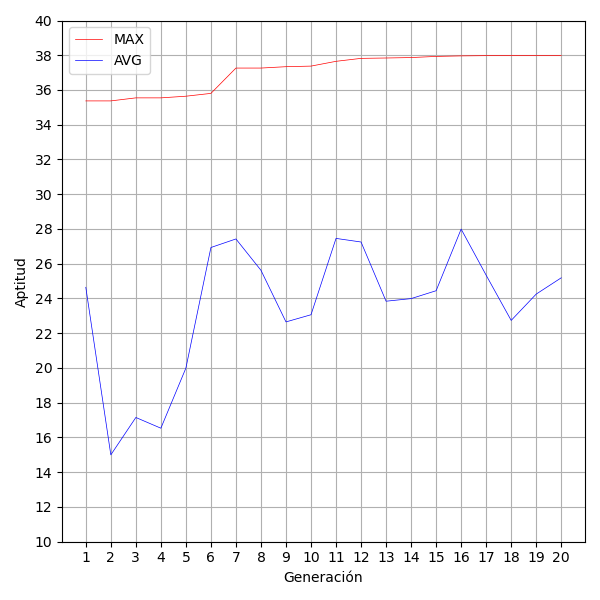
\includegraphics[width=.7\textwidth]{genetico/pop_evolution.png}
    \caption{Evolución de la primer optimización.}\label{fig:pop_ev_1}
\end{figure}

\begin{table}
  \centering
  \begin{tabular}{cc} \toprule
    Parámetro & Valor & Unidad \midrule
    DTA & 97.24 & mm\\
    DTE & 81.15 & mm\\
    LIT & 519.31 & mm\\
    LET & 976.66 & mm\\
    IIA & 1.12 & grado\\
    IFA & 70.15 & grado\\
    EIA & 85.14 & grado\\
    EFA & 11.13 & grado\\ \bottomrule
  \end{tabular}
  \caption{Mejor Candidato.}\label{tab:resultado_primer_it}
\end{table}


En la figura XXX se muestran las curvas de potencia y torque del motor, como es
de esperarse se ve que ambas copian la curva de rendimiento volumétrico, con una
potencia máxima de XXX HP a 1000 rpm y un torque máximo de xxxx N.m. a xxx rpm.

\subsection{Puerto de admisión}

Evaluando las curvas de presión para estas rpm se observa que durante la
apertura del puerto de escape hay una depresión de XXX Pa, para este punto el
coeficiente de descarga se estima en XXX y fluje un XX porciento de la masa
total que ingresa durante el período angular en que se encuentra abierto el
puerto.

El puerto de escape ocupa un período angular de $69^{\circ}$, inciando la
apertura en $1.12^{\circ}$ y cerrando a $70.15^{\circ}$ en relación al giro del
cigüeñal.

Se puede concluir que el puerto de admisión tiene sintonías en XXX, XXX, XXX rpm, siendo los diferenciales de presión mayores en xxx xxx xxx.

\subsection{Puerto de admisión}
%
El puerto de escape ocupa un período angular de $69^{\circ}$, inciando la
apertura en $1.12^{\circ}$ y cerrando a $70.15^{\circ}$ en relación al giro del cigüeñal.


\subsection{Modelo de CAD}
%
Los parámetros geométricos obtenidos se utilizaron para modelar los puertos,
tratando de generar una transición suave entre puerto y cámara de combustión
para favorecer el pasaje de gas.
%
Como se ve en la figura~\ref{fig:motor_cad}, se redondearon las aristas internas incluyendo las
paletas y las puntas del rotor, esto para favorecer el proceso de mallado
requerido en el paso siguiente a este ya que los bordes agudos son complejos de
adaptar a una malla construida con tetraedros, como lo es la malla resultante de
snappyHexMesh que se describió en el apartado xxx del capítulo xxx.

\begin{figure}
  \centering
    \begin{subfigure}{0.4\textwidth}
        \centering
        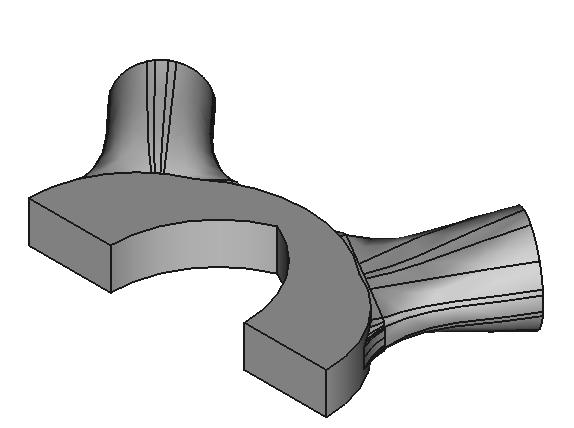
\includegraphics[width=\textwidth]{CAD/motor_cad1.png}
    \end{subfigure}
    \hfill
    \begin{subfigure}{0.4\textwidth}
        \centering
        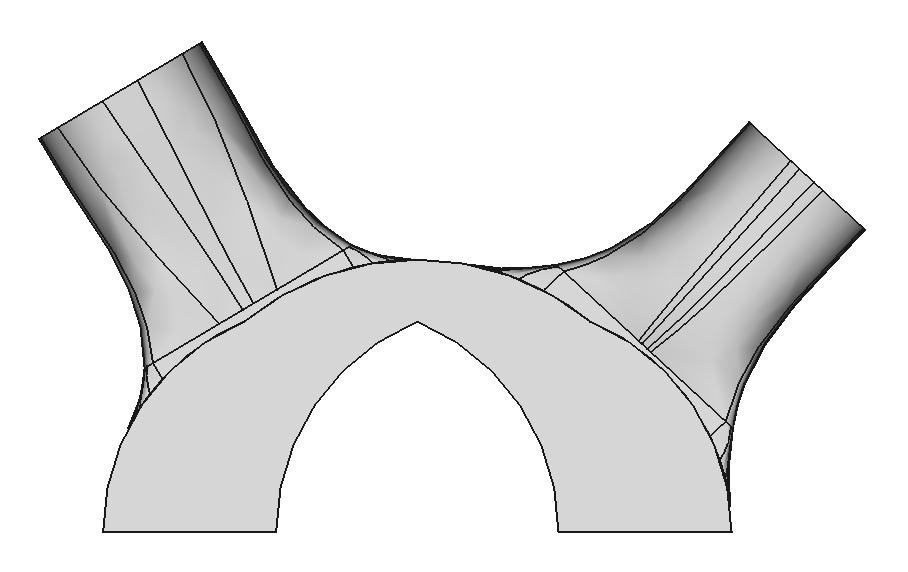
\includegraphics[width=\textwidth]{CAD/motor_cad2.png}
    \end{subfigure}
  \caption{CAD Primer Iteración}\label{fig:motor_cad1}
\end{figure}

La altura del puerto del lado de la cámara de combustión se mantuvo en dos
tercios del a altura de cámara.

\begin{figure}
  \centering
    \begin{subfigure}{0.8\textwidth}
        \centering
        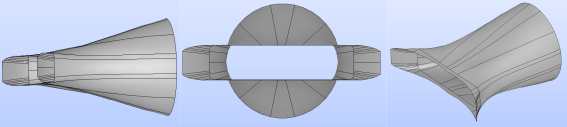
\includegraphics[width=\textwidth]{CAD/vistas_admision.png}
        \caption{Puerto de Admsisión.}
    \end{subfigure}
    \begin{subfigure}{0.8\textwidth}
        \centering
        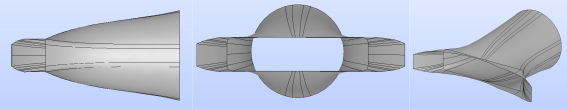
\includegraphics[width=\textwidth]{CAD/vistas_escape.png}
        \caption{Puerto de Escape.}
    \end{subfigure}
  \caption{CAD Primer iteración (vistas fuera de escala).}\label{fig:motor_cad2}
\end{figure}


\section{Flujometrías}

De los resultados de la primer otpimización se extrajo una curva de diferencia
de presión vs alzada para diferentes velocidades del motor para identificar los
puntos de mayor interés para realizar las fluometrías, tratando de obtener una
buena cobertura del rango de funcionamiento de cada puerto.

Inicialmente se propusieron un total de XXX flujometŕias, sin embargo algunas
combinaciones de $\l_{v}, \Delta P$ no se pudieron ejecutar hasta la
convergencia del flujo másico, por lo que se redujo la cantidad de flujometrías
final a xxx flujometrías, xxx para el puerto de admisión y xxx para el puerto de
escape, el par $(\l_{v}, \Delta P)$ se detalla en la figura XXX y tabla xxx.
%
Con estos datos se calculó el coeficiente de descarga para cada punto evaluado
obteniendo la base para generar el mapa de coeficientes de descarga que se
utilizará en el próximo paso de simulación, los valores de presión, alzada y
coeficiente de descarga obtenidos se listan en la tabla xxx.

Como se mencionó en el apartado~\ref{ch:mrcvc}, la modificaión realizada a
ICESym para funcionar con un mapa de $C_{D}$ dependiente de dos variables
requiere que los datos de entrada estén distribuidos en una grilla rectangular,
motivo por el cual a partir de estos valores se utilizó el método de
interpolación por IDW mencionado en el mismo apartado para generar una dicha
grilla de valores de $(l_{v}, \Delta P)$ con $C_{D}$ interpolado de los datos
conocidos, como se ve en las figuras~\ref{fig:mapa_cd_admision}
y~\ref{fig:mapa_cd_escape}.

\begin{figure}
    \centering
    \begin{subfigure}{0.4\textwidth}
        \centering
        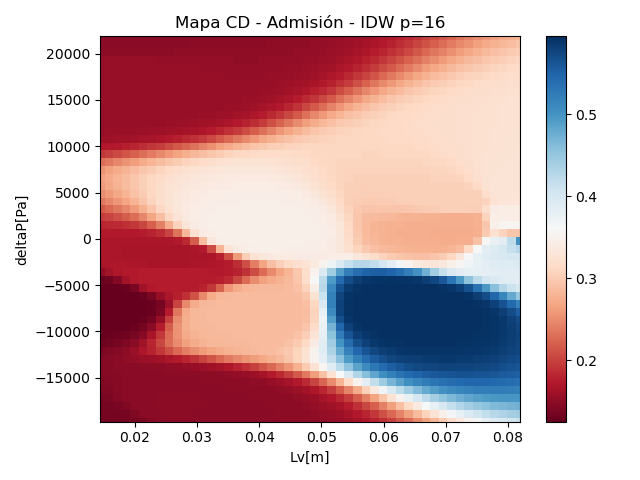
\includegraphics[width=\textwidth]{mapa_cd/idw16_mapa_adm.png}
        \caption{cambiar}
    \end{subfigure}
    \hfill
    \begin{subfigure}{0.4\textwidth}
        \centering
        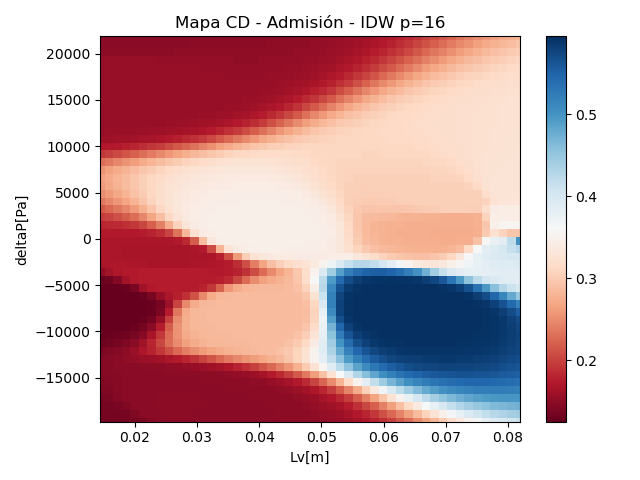
\includegraphics[width=\textwidth]{mapa_cd/idw16_mapa_adm.png}
        \caption{cambiar}
    \end{subfigure}
    \caption{cabmiar}\label{fig:mapa_cd_admision}
\end{figure}

\begin{figure}
    \centering
    \begin{subfigure}{0.4\textwidth}
        \centering
        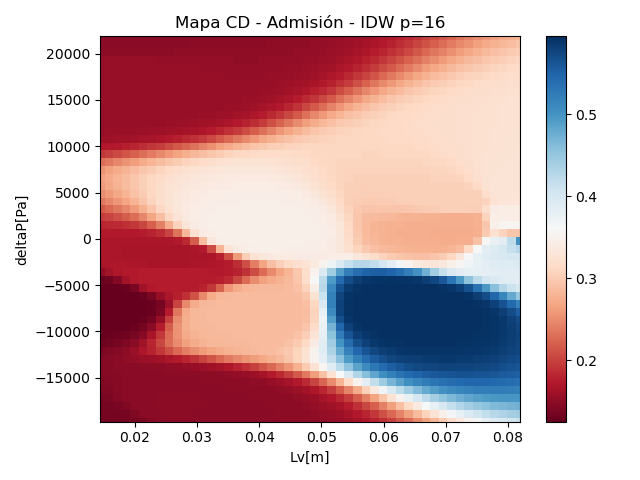
\includegraphics[width=\textwidth]{mapa_cd/idw16_mapa_adm.png}
        \caption{cambiar}
    \end{subfigure}
    \hfill
    \begin{subfigure}{0.4\textwidth}
        \centering
        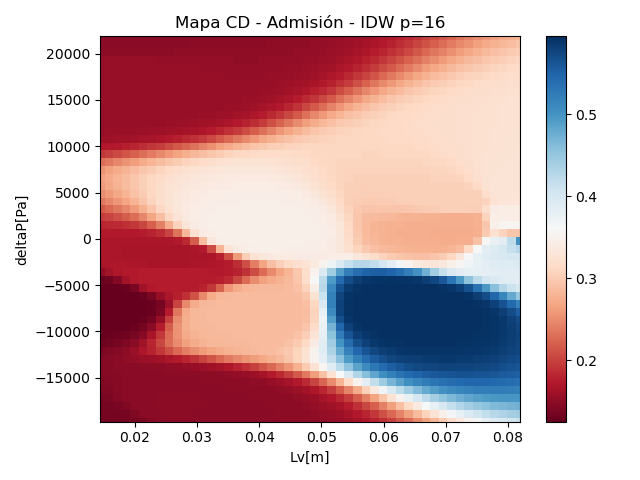
\includegraphics[width=\textwidth]{mapa_cd/idw16_mapa_adm.png}
        \caption{cambiar}
    \end{subfigure}
    \caption{cabmiar}\label{fig:mapa_cd_escape}
\end{figure}

En el mapa del puerto de admisioń se observa un máximo para para aperturas del
puerto mayores a 80mm, con $\Delta P$ de entre 1000 Pa a 15000 Pa.
%
El coefiente de descarga máximo es $C_{D}(100mm, 1500Pa) = 0.6$ y corresponde a
la flujometría $N^{\circ} X$, el flujo másico obtenido para este régimen es de
0.02 kg/s, con un a velocidad máxima de xxx m/s en la garganta.
%
El peor valor se es $C_{D}(100mm, 1500Pa) = 0.6$ y corresponde a aperturas
pequeñas del puerto, en la que debido a la reducida sección de pasaje de flujo
se tiene velocidades eleveadas, siendo la máxima de xxx m/s.
%
Para visualizar la diferencia entre uno y otro caso, se representan las líneas
de corriente para ambos casos en la figura \ref{fig:comparativa_lineas_corriente}.

\begin{figure}
    \centering
    \begin{subfigure}{0.4\textwidth}
        \centering
        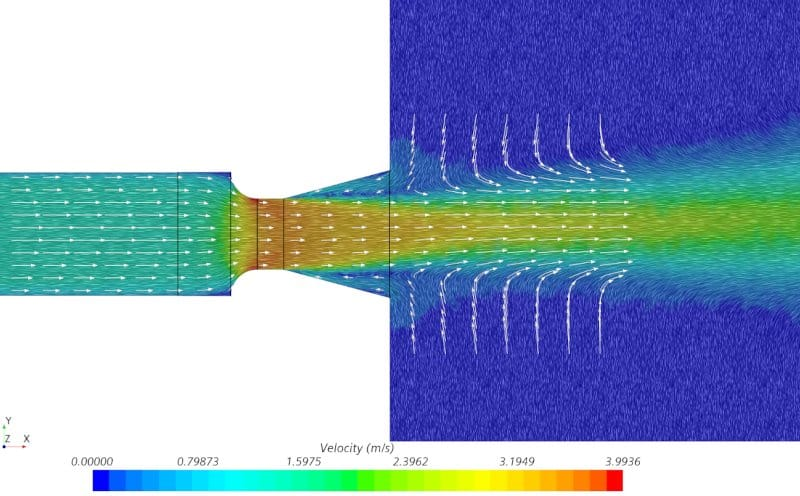
\includegraphics[width=\textwidth]{flujometrias/ejemplo_lineas_corriente.jpg}
        \caption{Valor máximo de $C_{D}$}
    \end{subfigure}
    \hfill
    \begin{subfigure}{0.4\textwidth}
        \centering
        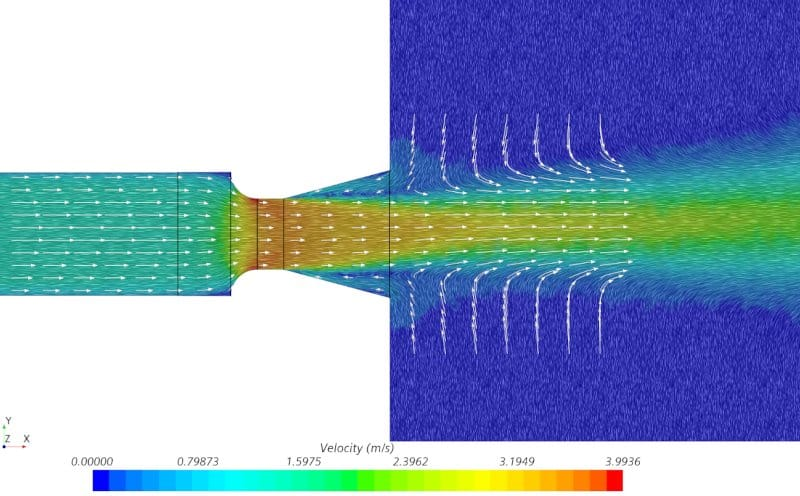
\includegraphics[width=\textwidth]{flujometrias/ejemplo_lineas_corriente.jpg}
        \caption{Valor mínimo de $C_{D}$}
    \end{subfigure}
    \caption{cabmiar}\label{fig:comparativa_lineas_corriente}
\end{figure}

Para el mapa del puerto de escape se observa un máximo para para aperturas del
puerto mayores a 80mm, con $\Delta P$ de entre 1000 Pa a 15000 Pa.
%
El coefiente de descarga máximo es $C_{D}(100mm, 1500Pa) = 0.6$ y corresponde a
la flujometría $N^{\circ} X$, el flujo másico obtenido para este régimen es de
0.02 kg/s, con un a velocidad máxima de 10m/s en la garganta, como se ve en la
figura \ref{fig:admision_10_2000.jpg}.

\begin{figure}
    \centering
    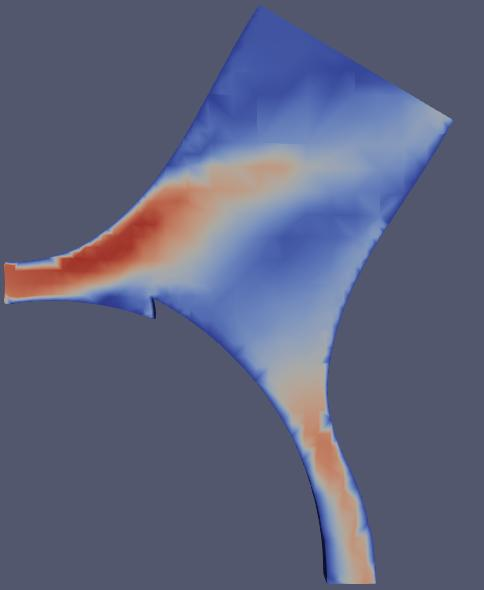
\includegraphics[width=0.7\textwidth]{flujometrias/admision_10_2000.jpg}
    \caption{Puerto de admisión - $10^{\circ}$@2000 RPM}\label{fig:admision_10_2000.jpg}
\end{figure}

El peor valor se es $C_{D}(100mm, 1500Pa) = 0.6$ y corresponde a aperturas
pequeñas del puerto, en la que debido a la reducida sección de pasaje de flujo
se tiene velocidades eleveadas, siendo la máxima de xxx m/s.
%
Para visualizar la diferencia entre uno y otro caso, se representan las líneas
de corriente para ambos casos en la figura \ref{fig:admision_10_2000.jpg}.

\begin{figure}
    \centering
    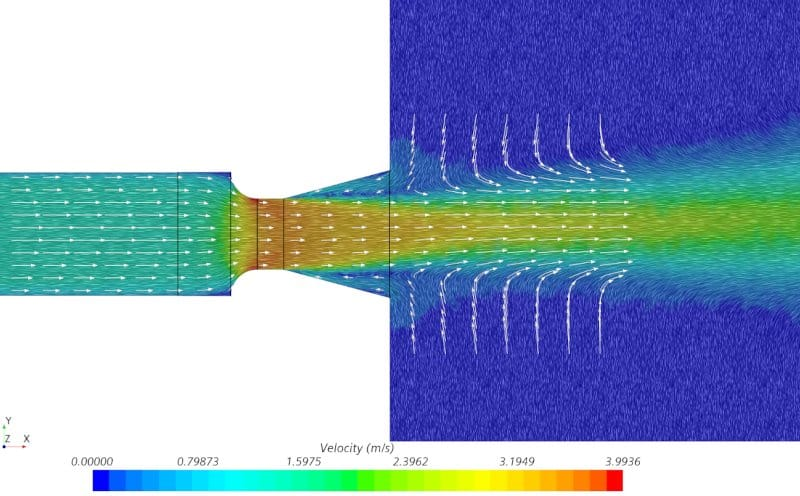
\includegraphics[width=0.7\textwidth]{flujometrias/ejemplo_lineas_corriente.jpg}
    \caption{Puerto de admisión - $10^{\circ}$@2000 RPM}\label{fig:admision_10_2000.jpg}
\end{figure}

En las tablas~\ref{tab:mapa_cd_admision} y~\ref{tab:mapa_cd_escape} se muestran los
resultados de realizar las flujometrías de los puertos de admisión y escape.

\begin{table}
  \centering
    \begin{tabular}{cccc} \toprule
      Caso  & lv        & $\Delta P$    & $C_{D}$   \\ \midrule
      0     & 0.016826  & -100331.39    &  0.213882 \\
      0     & 0.106775  & 5723.72       &  0.489375 \\
      0     & 0.016826  & -263797.72    &  0.011021 \\
      0     & 0.106775  & -3296.18      &  0.803197 \\
      0     & 0.016826  & -652902.78    &  0.011106 \\
      0     & 0.106775  & -9613.29      &  0.815804 \\
      0     & 0.016826  & -513568.73    &  0.011280 \\
      0     & 0.106775  & -3232.97      &  0.813186 \\
      1     & 0.026960  & -116996.12    &  0.375219 \\
      1     & 0.096641  & -3643.9       &  0.878414 \\
      1     & 0.026960  & -237724.11    &  0.018632 \\
      1     & 0.096641  & -6684.11      &  0.867774 \\
      1     &  0.02696  & -496509.46    &  0.111212 \\
      1     &  0.09664  & -18256.20     &  0.805830 \\
      1     & 0.026960  & -237724.11    &  0.022716 \\
      1     & 0.096641  & -6684.11      &  0.862647 \\
      2     & 0.047228  & -49343.47     &  0.541857 \\
      2     & 0.076373  & -5712.86      &  0.918061 \\
      2     & 0.047228  & -109348.67    &  0.487137 \\
      2     & 0.076373  & -17090.38     &  0.914182 \\
      3     & 0.067496  & 13.83         &  0.696967 \\
      3     & 0.071759  & -134.24       &  0.707263 \\
      3     & 0.067496  & -100073.52    &  0.731100 \\
      3     & 0.071759  & -24077.34     &  0.723965 \\
      4     & 0.075750  & -11793.31     &  0.946392 \\
      4     & 0.087764  & -33418.12     &  0.235717 \\
      4     & 0.087764  & -10715.70     &  0.221632 \\
      4     & 0.075750  & -5167.81      &  0.897169 \\
      6     & 0.123601  & -73.94        &  0.878522 \\ \bottomrule
    \end{tabular}
  \caption{Mapa de Cd del puerto de escape} \label{tab:mapa_cd_escape}
\end{table}

\begin{table}
  \centering
  \begin{tabular}{cccc} \toprule
      Caso  & lv        & $\Delta P$    & $C_{D}$   \\ \midrule
      0     & 0.014432  & -6574.97      &  0.206543 \\
      0     & 0.081937  & -87.24        &  0.828822 \\
      0     & 0.014432  & 21856.29      &  0.243975 \\
      0     & 0.081937  & -573.65       &  0.738459 \\
      0     & 0.014432  & -19738.67     &  0.222406 \\
      0     & 0.081937  & 519.60        &  0.487115 \\
      0     & 0.081937  & 1571.95       &  0.587277 \\
      0     & 0.014432  & 18077.97      &  0.256415 \\
      0     & 0.014432  & 2668.61       &  0.247292 \\
      0     & 0.081937  & 0.98          &  0.025970 \\
      2     & 0.062951  & -297.79       &  0.816487 \\
      2     & 0.081937  & 292.92        &  0.466147 \\
      2     & 0.062951  & -7374.88      &  0.980617 \\
      2     & 0.081937  & 4953.85       &  0.541619 \\
      3     & 0.071763  & 4092.13       &  0.501641 \\
      3     & 0.025832  & -3689.81      &  0.289852 \\
      4     & 0.069767  & -789.00       &  0.615690 \\
      4     & 0.069767  & 7869.92       &  0.599348 \\
      4     & 0.005564  & -12539.15     &  0.534555 \\
      4     & 0.005564  & -10091.84     &  0.583979 \\ \bottomrule
    \end{tabular}
  \caption{Mapa de Cd del puerto de Admisión} \label{tab:mapa_cd_admision}
\end{table}


La geometría obtenida luego de realizar la optimización con los mapas de Cd
incorporados a la simulación de ICESym se muestra en la figura \ref{fig:geom_nueva}.
%
Se puede ver que la geometría es similar a la inicial, siendo el puerto de
admisión algo menor en cuanto a diámetro que en el caso inicial.

Como es de esperarse, incorporar estos mapa al modelo del motor tiene un efecto
en el comportamiento del mismo, esto se puede observar principalmente en las
curvas de presión del motor.

\section{Segunda Iteración}

\chapter{Conclusiones}
Falta


% -- Finales
\printbibliography
\include{partes/apendices}
\end{document}
